\section{Defenisi Konversi Bilangan}
Konversi bilangan merupakan suatu proses yang mana satu system bilangan dengan basis khusus tau tertentu akan dibuat menjadi bilangan dengan basis yang lainnya. 
Yaitu dengan cara membagikan bilangan yang desimal dengan dua dan kemudian diambil sisa pembagiannya.
caranya dengan mengalikan masing-masing bit pada bilangan dengan posisi nilainya.
\\Didalam dunia perkomputer kita dapat mengenal empat macam-macam bilangan , seperti bilangan biner,bilangan oktal, bilangan desimal , dan yang terakhir adalah bilangan hexadesimal.
\section{Konversi bilangan biner}
\subsection{Bilangan Biner}
Sistem bilangan biner merupakan sistem dengan penulisan angka yaitu 0 dan 1.Sistem bilangan biner  modern ditemukan oleh Gittfried Wilhem Leibniz pada abad ke 17. Sistem biner juga biasa disebut dengan bit atau,Binary digit.
\subsection{Konsep Bilangan Biner}
Bilangan biner menggunakan metode yang berkaitan dengan basis,bilangan biner juga menggunakan berbasis 2. Adapun contoh biner sebagai berikut : \\
\begin{itemize}
\item 1110(2) = (1x23)+(1x22)+(1x21)+(0x20)\\
   	  = 8+4+2+0\\
             = 14  
\end{itemize}

\section{Bilangan Oktal} %Septia Rahayu (26-10-2017)
Bilangan oktal adalah sistem bilangan yang berbasis 8 dan mempunyai delapan simbol bilangan yang berbeda : 0,1,2,...,7.
\\
	Teknik pembagian yang berurutan dapat menggunakan untuk mengubah bilangan desimal menjadi bilangan oktal. Bilangan desimal yang akan diubah secara berturut-turut dibagi dengan 8 dan sisa pembagian harus selalu dicatat. Sebagai contoh, untuk mengubah bilangan 5819.10 ke oktal.

\section{Bilangan Desimal} Salwaa Tania (26-10-2017)
Bilangan desimal adalah bilangan yang menggunakan 10 angka mulai 0 sampai 9 berturut-turut. Setelah angka 9 , maka angka berikutnya adalah 10,11,12 dan seterusnya. Bilangan desimal disebut juga dengan bilangan berbasis 10.
\\Contoh: 1710
\\Berikut bagaimana cara melakukan konversi antar basis bilangan: 
\begin{itemize}
	\item Cara Konversi desimal ke basis lainnya
	\item Konversi desimal ke biner
	\item Konversi desimal ke Oktal
	\item Konversi desimal ke Heksadesimal
\end{itemize}
\subsection{Cara mengkoversikan bilangan desimal ke biner}
\begin{figure}[ht]
\centerline{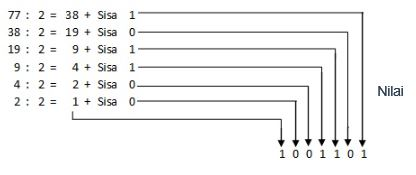
\includegraphics[width=1\textwidth]{figures/konversibiner.JPG}}
\caption{Cara mengkonversikan bilangan desimal ke biner}
\label{Contoh Konversi Bilangan Desimal}
\end{figure}
Seperti yang bisa kita lihat pada \ref{konversibiner} bahwa cara mengkonversikan bilangan desimal ke dalam bilangan biner adalah dengan membagi bilangan desimal dengan nilai 2 (basis). Cara ini merupakan cara yang sering digunakan oleh banyak orang dan cara ini cukup mudah untuk di pahami dan diterapkan.  


\section{Fungsi dari Konversi Bilangan} %Luthfi Muhammad Nabil (25-10-2017)
Fungsi dari Konversi bilangan ini salah satunya adalah untuk membaca sebuah perintah yang dimana perintah tersebut masih menggunakan perintah yang hanya bisa dibaca oleh komputer yaitu Biner. tetapi dengan adanya Konversi Bilangan, Sebuah angka tersebut bisa dijadikan sebagai suatu line perintah bahkan sebuah kata yang nantinya dapat dimunculkan oleh komputer kepada pengguna. Pembuatan aplikasi sendiri membutuhkan sebuah Konversi Bilangan yang nantinya akan menggerakan sebuah modul - modul dalam sebuah perangkat yang dipakai dalam aplikasi tersebut. 

\section{Penerapan Konversi Bilangan} %Luthfi Muhammad Nabil (26-10-2017)
Konversi Bilangan diterapkan khususnya pada bidang Teknologi. Selain sebagai instruksi, Konversi sendiri dapat dikenal sebagai pengenal dalam situasi tertentu. seperti untuk mengenal warna dan sebagainya. Beberapa contoh dari penerapan tersebut adalah sebagai berikut : 
\begin{itemize}
	\item Sebagai kode warna dalam pemrograman \\ Konversi Bilangan sering sekali dipakai untuk mengetahui berapa tingkat warna dan seberapa pekat warna tersebut. Konversi Bilangan pada kasus ini menggunakan Konversi Desimal ke Heksadesimal dimana warna terbagi menjadi Merah, Hijau, Biru. 
\end{itemize}

%Note : Setiap mau push kasih note atau attention biar diarahkan supaya sebelum push nanti di pull dulu biar tau siapa yang mau push (Komunikasi Tetap Terjaga)
